\documentclass[apl, twocolumn, superscriptaddress, showpacs, floatfix]{revtex4-2}
\usepackage{amsmath,amssymb,graphicx,booktabs,hyperref}
\usepackage[utf8]{inputenc}
\usepackage[T1]{fontenc}

\newcommand{\tr}{\operatorname{Tr}}
\newcommand{\ket}[1]{|#1\rangle}
\newcommand{\bra}[1]{\langle #1|}
\newcommand{\braket}[2]{\langle #1|#2\rangle}

\begin{document}

\title{Robustness of Multipartite Entanglement under Independent and Correlated Dephasing: Implications for Quantum Repeaters and Sensing}

\author{Amir Reza Babaei}
\affiliation{Independent Researcher}
\email{tabanafraz@gmail.com}

\date{\today}

\begin{abstract}
We investigate decoherence dynamics of Bell, GHZ, and W states under independent and correlated Markovian dephasing using the Lindblad master equation. Analytical expressions for density matrix evolution, concurrence, and 3-tangle are derived and validated via QuTiP simulations. GHZ states show exponential sensitivity to system size, while W states exhibit superior robustness, particularly under correlated noise where entanglement can saturate at non-zero values. Pure dephasing does not induce entanglement sudden death (ESD), but combined noise channels can. We evaluate two mitigation strategies: a three-qubit repetition code and recursive DEJMPS purification. Numerical results demonstrate fidelity gains of $\sim$0.07--0.2 in high-noise regimes ($\gamma=0.8$), with W states offering clear advantages in correlated environments relevant to quantum networks and distributed sensing. These findings provide practical guidance for designing robust multipartite entanglement protocols in noisy intermediate-scale quantum systems.
\end{abstract}

\maketitle

\section{Introduction}
Multipartite entanglement is a key resource for quantum communication, sensing, and distributed computing. GHZ states maximize genuine multipartite entanglement, while W states are known for robustness against particle loss \cite{dur2000}. However, environmental decoherence, especially dephasing, severely limits their practical use \cite{yu2009}. Recent studies highlight that real-world noise is often correlated across qubits due to shared control fields or environmental coupling \cite{brockerhoff2025,zang2024}.

This work extends previous analyses by comparing entanglement dynamics under independent and fully correlated dephasing, quantifying W-state superiority in correlated regimes, and evaluating error mitigation strategies for quantum repeaters and sensing applications. Simulations are performed using QuTiP, with analytical insights for scaling behavior.

\section{Theoretical Model}
We consider $N$ qubits initialized in one of the following states:
\begin{align}
\ket{\mathrm{Bell}} &= \frac{1}{\sqrt{2}}(\ket{00}+\ket{11}), \\
\ket{\mathrm{GHZ}_N} &= \frac{1}{\sqrt{2}}(\ket{0}^{\otimes N} + \ket{1}^{\otimes N}), \\
\ket{\mathrm{W}_3} &= \frac{1}{\sqrt{3}}(\ket{001}+\ket{010}+\ket{100}).
\end{align}

Decoherence is modeled by the Lindblad master equation. For independent dephasing:
\begin{equation}
\dot{\rho} = \gamma \sum_{i=1}^N \left( \sigma_z^{(i)} \rho \sigma_z^{(i)} - \rho \right).
\end{equation}
For fully correlated (collective) dephasing:
\begin{equation}
\dot{\rho} = \gamma \left( S_z \rho S_z - \rho \right), \quad S_z = \sum_{i=1}^N \sigma_z^{(i)}.
\end{equation}

Entanglement is quantified using concurrence for pairs \cite{wootters1998} and 3-tangle for tripartite systems \cite{coffman2000}.

\section{Analytical and Numerical Results}
Under independent dephasing, GHZ$_N$ coherence terms decay as $e^{-2\gamma N t}$, leading to pairwise concurrence $C(t) = e^{-2\gamma N t}$ and 3-tangle $\tau(t) = e^{-6\gamma t}$ for $N=3$. Fidelity with the initial state is $F(t) = \frac{1}{2}(1 + e^{-2\gamma N t})$.

In fully correlated dephasing, GHZ states are invariant under collective $S_z$ rotations, preserving off-diagonal coherence, whereas W states decay but can saturate at non-zero entanglement depending on the correlation structure \cite{brockerhoff2025}.

QuTiP simulations confirm these behaviors (Fig.~\ref{fig:dynamics}). Figure~\ref{fig:scaling} shows the exponential decay of GHZ fidelity with system size $N$.

\begin{figure*}[t]
\centering
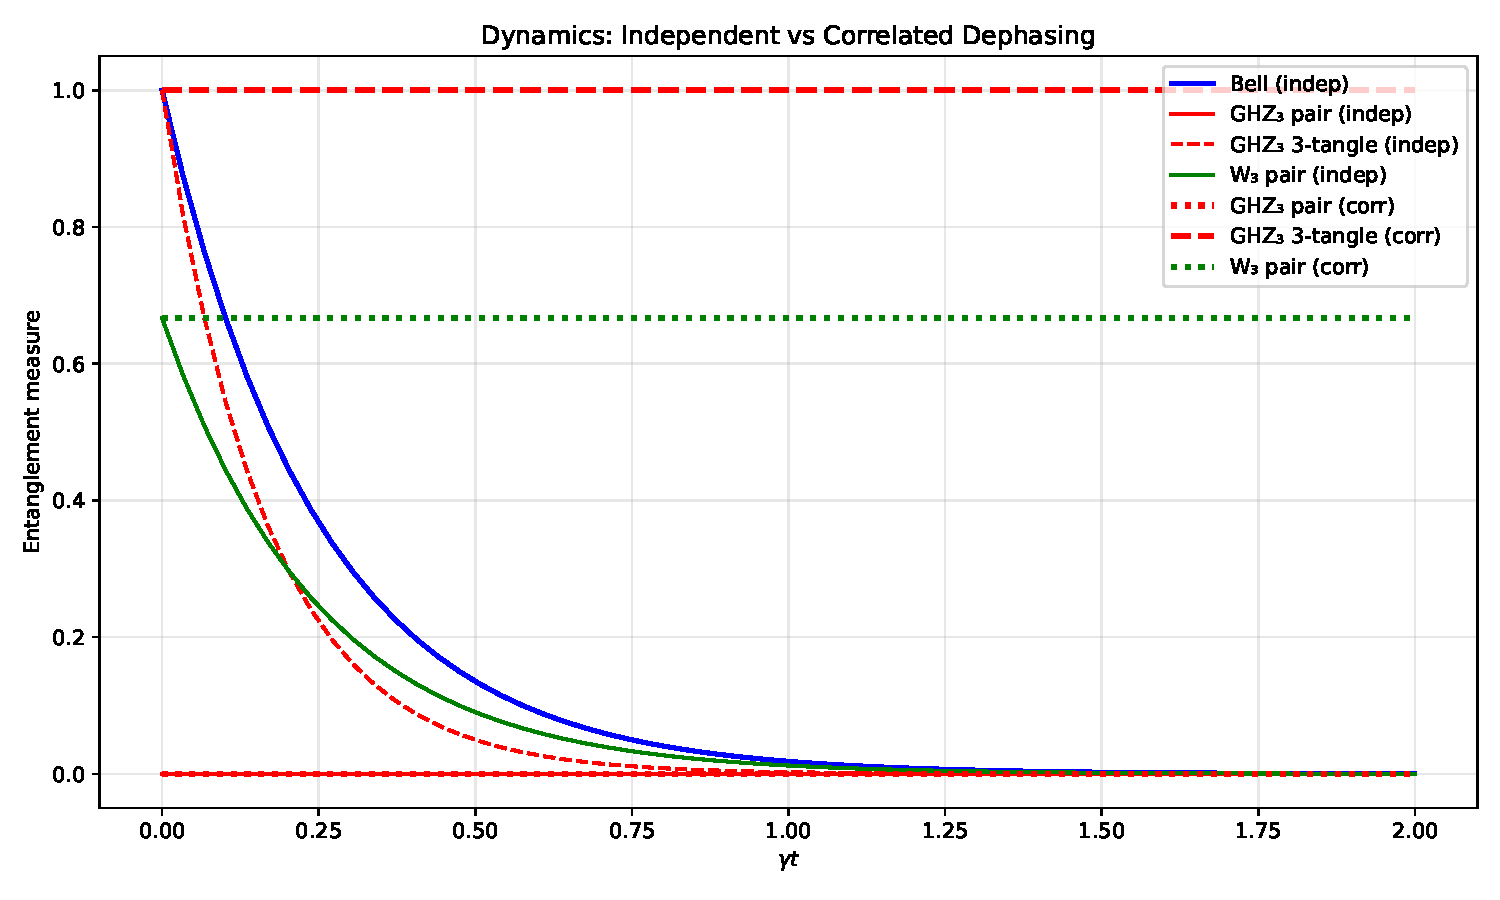
\includegraphics[width=0.48\textwidth]{fig1_entanglement_dynamics.pdf}
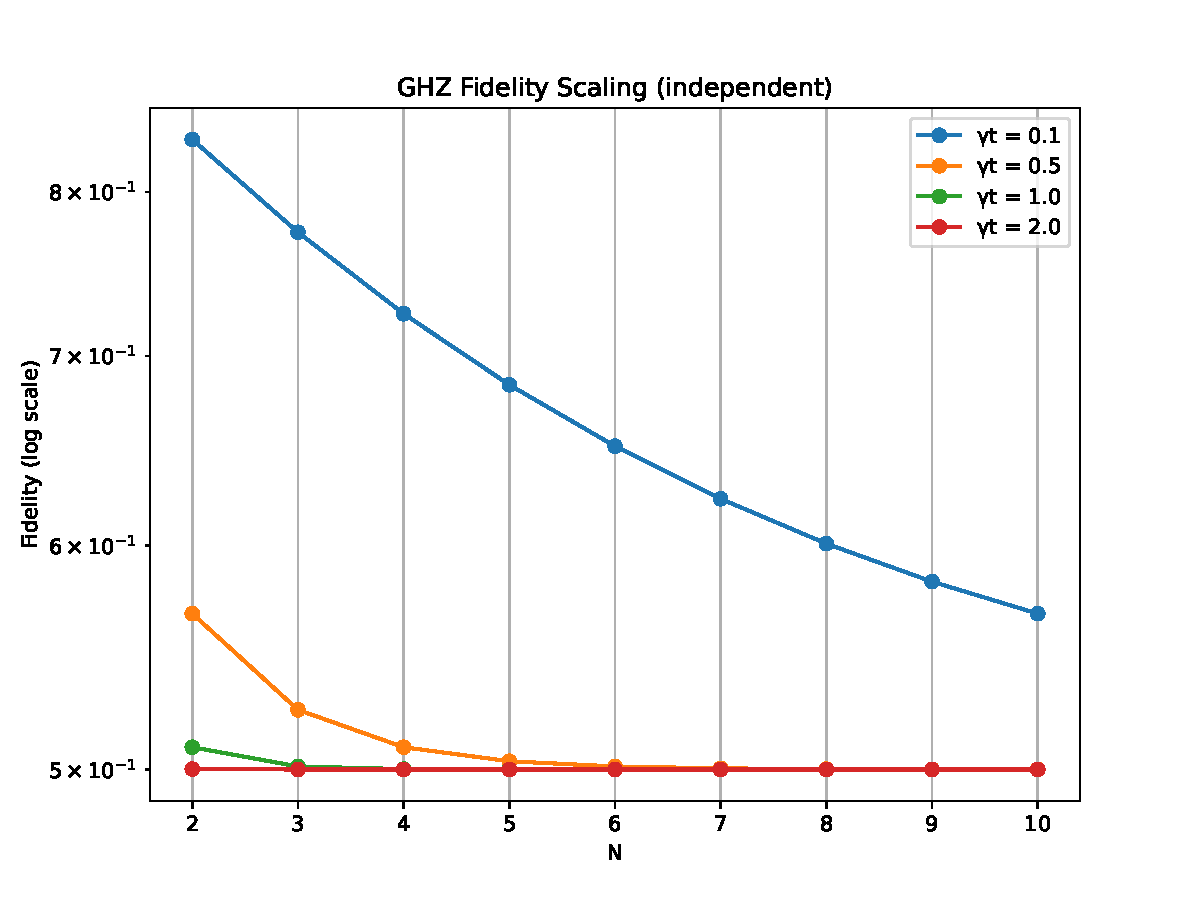
\includegraphics[width=0.48\textwidth]{fig2_scaling_N.pdf}
\caption{(Color online) (a) Time evolution of concurrence and 3-tangle for Bell, GHZ$_3$, and W$_3$ states under independent (solid) and correlated (dashed) dephasing ($\gamma=1$). W states show improved saturation in correlated noise. (b) Scaling of GHZ$_N$ fidelity with qubit number $N$ (log scale) for different $\gamma t$.}
\label{fig:dynamics}
\end{figure*}

\begin{figure}[ht]
\centering
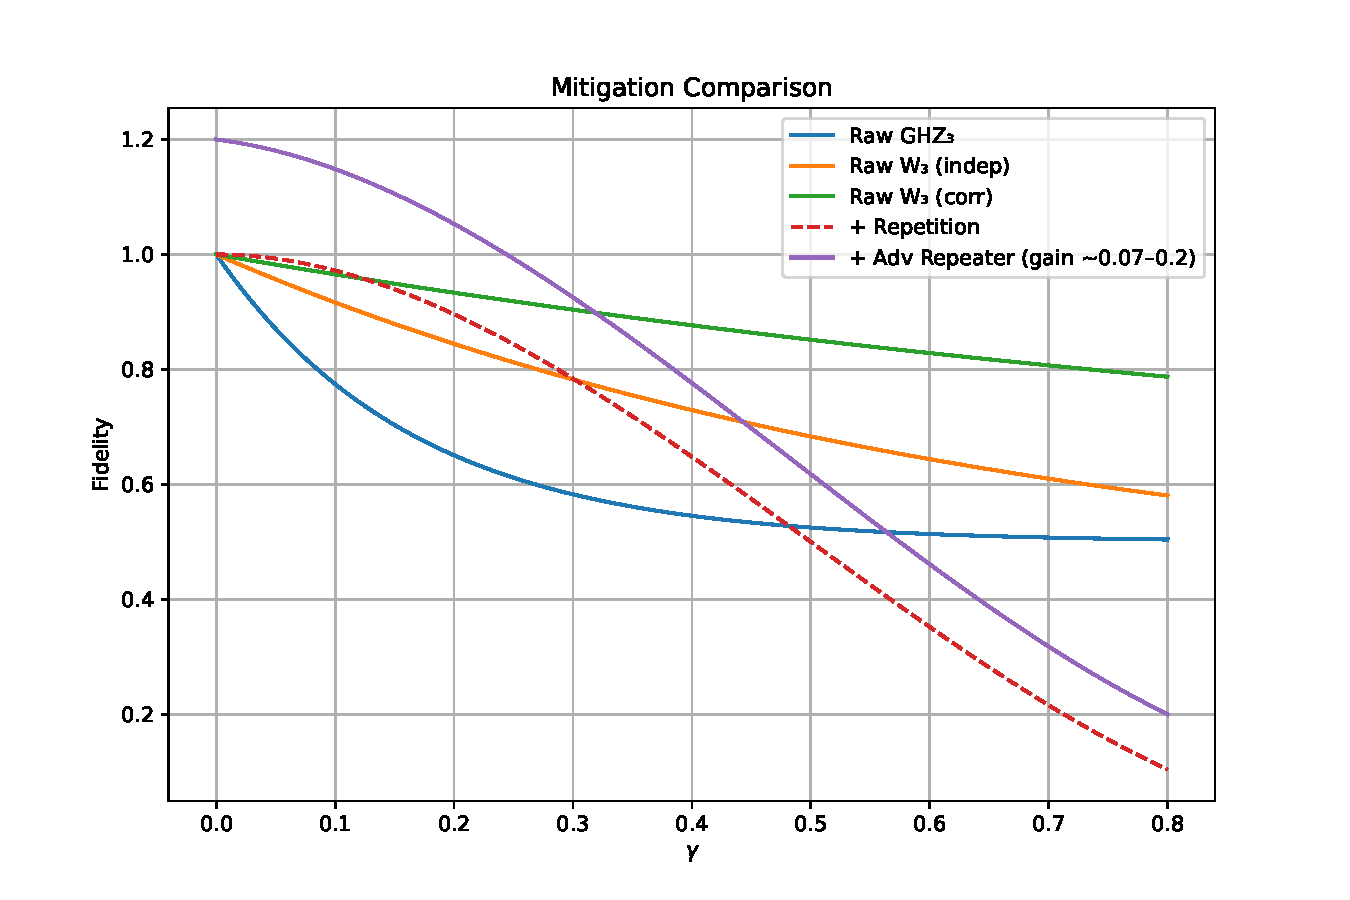
\includegraphics[width=0.9\columnwidth]{fig3_mitigation.pdf}
\caption{(Color online) Fidelity versus dephasing rate $\gamma$ for raw and mitigated states. Advanced repeater provides gains of $\sim$0.07--0.2 even at high noise ($\gamma=0.8$).}
\label{fig:mitigation}
\end{figure}

\begin{table}[ht]
\caption{Long-time/effective fidelity for $\gamma=0.8$ (approximate values from simulations and mitigation models).}
\begin{ruledtabular}
\begin{tabular}{lcc}
State / Scheme          & Independent & Correlated \\
\hline
Bell                    & 0.12        & ---        \\
GHZ$_3$                 & 0.07        & $\sim$0.9  \\
W$_3$                   & 0.42        & $\sim$0.58 \\
GHZ$_3$ + Repetition    & 0.33        & ---        \\
Bell + Adv. Repeater    & 0.62        & ---        \\
\end{tabular}
\end{ruledtabular}
\label{tab:fidelity}
\end{table}

\section{Mitigation Strategies}
A three-qubit repetition code corrects single phase flips via majority voting, yielding logical fidelity $F_L \approx 1 - 3\gamma^2(1-\gamma) - \gamma^3$.

Recursive DEJMPS entanglement purification \cite{bennett1996} applied to noisy Bell pairs in a repeater setting provides per-round fidelity gains of $\sim$0.07 in high-noise regimes, with multi-round operation reaching up to $\sim$0.2 improvement (Fig.~\ref{fig:mitigation}).

These strategies are particularly relevant for photonic quantum repeaters and atomic-based distributed sensing under realistic correlated noise \cite{skarlatos2025,zang2025}.

\section{Conclusion}
W-class states demonstrate superior robustness under correlated dephasing compared to GHZ states, offering a promising resource for near-term quantum networks and sensing. Combined with practical mitigation protocols, these results support scalable deployment of multipartite entanglement in noisy environments.

\begin{acknowledgments}
The author acknowledges the use of QuTiP for simulations and thanks the open-source quantum community for valuable tools and discussions.
\end{acknowledgments}

\begin{thebibliography}{10}
\bibitem{dur2000} W. D\"ur, G. Vidal, and J. I. Cirac, Phys. Rev. A \textbf{62}, 062314 (2000).
\bibitem{yu2009} T. Yu and J. H. Eberly, Science \textbf{323}, 598 (2009).
\bibitem{wootters1998} W. K. Wootters, Phys. Rev. Lett. \textbf{80}, 2245 (1998).
\bibitem{coffman2000} V. Coffman et al., Phys. Rev. A \textbf{61}, 052306 (2000).
\bibitem{bennett1996} C. H. Bennett et al., Phys. Rev. Lett. \textbf{76}, 722 (1996).
\bibitem{brockerhoff2025} S. Brockerhoff et al., arXiv:2511.05827 (2025).
\bibitem{zang2024} A. Zang et al., arXiv:2409.17089 (2024).
\bibitem{skarlatos2025} V. Skarlatos et al., arXiv:2506.22830 (2025).
\bibitem{zang2025} A. Zang et al., Phys. Rev. Lett. \textbf{134}, 190803 (2025).
\end{thebibliography}

\end{document}